\documentclass{beamer}
\usepackage{graphicx}
\usepackage{paralist}
\usepackage{outlines}

\title{Lasso Tools}
\author{Mendocino College - Image Manipulation with Photoshop}
\titlegraphic{\vspace{-10mm}
\includegraphics[width = .8\textwidth]{images/photoshop.jpg}} 
\date{\vspace{-5em}} 


\mode <presentation>
\usetheme{Warsaw}
\usecolortheme{default}

\setbeamerfont{footline}{size=\fontsize{5}{8}\selectfont}

\definecolor{darkred}{rgb}{20,0,0}
\definecolor{darkgreen}{RGB}{40,110,20}
\definecolor{darkpurple}{RGB}{30,0,30}
\definecolor{chardonnay}{RGB}{255, 255, 204}

\setbeamercolor*{palette primary}{fg=white, bg=darkgreen}


\begin{document}
	{
		\setbeamertemplate{footline}{} 
		\setbeamertemplate{headline}{} 
		\begin{frame}
			\vspace{-35pt}
			\maketitle
		\end{frame}
	}


\section{Lasso Tool}
\begin{frame}
	\frametitle{Lasso Tool}
	\begin{center}
		
\includegraphics[width = 1.0\textwidth]{images/photoshop-lasso-selection.jpg}
	\end{center}
\end{frame}

\subsection{What is the Lasso Tool?}		
\begin{frame}
	\frametitle{What is the Lasso Tool?}
	\begin{outline}
		\1 The Lasso tool is useful for drawing freeform segments of a selection border.
		\1 The Rectangular Marquee Tool allows us to easily draw selections based on simple rectangular or square shapes, and  the Elliptical Marquee Tool extends our selection making abilities into ovals and circles. 
		\1 But what if we need to select something in a photo that's a little more complex, like someone's eyes, an item of clothing, or maybe a car or a bottle? 		
		\1 More advanced Photoshop users will probably head straight for the Pen Tool, the tool of choice for making professional quality form-based selections. 
		\1 But if you have a good quality mouse (or even better, a pen tablet), decent drawing skills and a little patience, you may find that the Lasso Tool, another of Photoshop's basic selection tools, is all you need.
	\end{outline}
\end{frame}

\subsection{How to use the Lasso Tool}		
\begin{frame}
	\frametitle{How to use the Lasso Tool}
	\begin{outline}
		\1 Drag to draw a freehand selection border.
		\1 To close the selection border, release the mouse.
		\1 Press Alt To switch between freehand and straight-edged segments, and click where segments should begin and end. 
	\end{outline}
	\begin{center}
	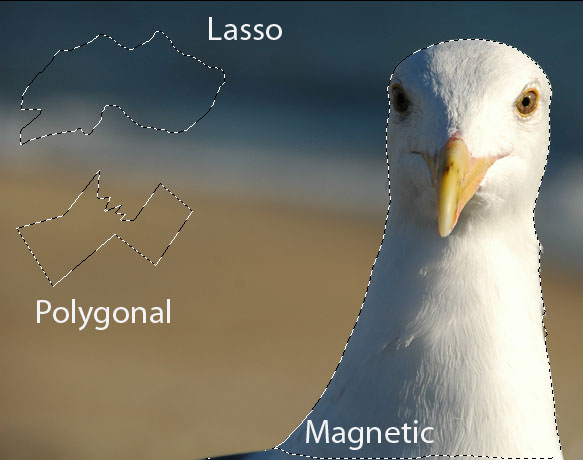
\includegraphics[width = 0.7\textwidth]{images/lasso_samples.jpg}
\end{center}
\end{frame}

\subsection{Lasso Tool Options}		
\begin{frame}
	\frametitle{Lasso Tool Options}
	\begin{outline}
		\1 Feathering
		\2 Blurs edges by building a transition boundary between the selection and its surrounding pixels. 
		\3 This blurring can cause some loss of detail at the edge of the selection.
		\1 Anti-aliasing
		\2 Smooths the jagged edges of a selection by softening the color transition between edge pixels and background pixels. 
		\3 No detail is lost, only the edge pixels change. 
		\3 Useful when cutting, copying, and pasting selections to create composite images.
	\end{outline}
	\begin{center}
		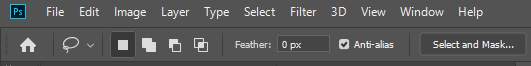
\includegraphics[width = 0.7\textwidth]{images/Lasso Options.png}
	\end{center}
\end{frame}


\section{Polygonal Lasso Tool}	
\subsection{Polygonal Lasso Tool}		
\begin{frame}
	\frametitle{Polygonal Lasso Tool}
	\begin{outline}
		\1 The Polygonal Lasso tool is useful for drawing straight-edged segments of a selection border.
		\1 To draw a straight segment, position the pointer where you want the first straight segment to end, and click. Continue clicking to set endpoints for subsequent segments.
		\1 Hold down Shift to draw a straight line at a multiple of 45°.
		\1 Press Delete to erase recently drawn straight segments.
		\1 To close your selection area, Position the Polygonal Lasso tool pointer over the starting point and click.
	\end{outline}
\end{frame}


\section{Magnetic Lasso Tool}	
\subsection{Magnetic Lasso Tool}		
\begin{frame}
	\frametitle{Magnetic Lasso Tool}
	\begin{outline}
		\1 When you use the Magnetic Lasso tool, the border snaps to the edges of defined areas in the image. 
		\1 The Magnetic Lasso tool is especially useful for quickly selecting objects with complex edges set against high-contrast backgrounds.
		\1 Note: The Magnetic Lasso tool is not available for 32‑bits-per-channel images.
	\end{outline}
	\begin{center}
	\includegraphics[width = 1.0\textwidth]{images/Magnetic Lasso1.png}
\end{center}
\end{frame}

\subsection{Magnetic Lasso Tool - Options}		
\begin{frame}
	\frametitle{Magnetic Lasso Tool - Options}
	\begin{outline}
		\1 Width
		\2 Detects edges only within the specified pixel width distance from the pointer. 
		\1 Contrast
		\2 To specify the lasso’s sensitivity to edges in the image, enter a value between 1\% and 100\% for Contrast. A higher value detects only edges that contrast sharply with their surroundings; a lower value detects lower-contrast edges.
		\1 Frequency
		\2 To specify the rate at which the lasso sets fastening points, enter a value between 0 and 100 for Frequency. A higher value anchors the selection border in place more quickly.
		\1 Stylus Pressure
		\2 If you are working with a stylus tablet, select or deselect the Stylus Pressure option. When the option is selected, an increase in stylus pressure decreases the edge width.
	\end{outline}
	\begin{center}
		\includegraphics[width = 1.0\textwidth]{images/Magnetic Lasso.png}
	\end{center}
\end{frame}



	
\end{document}